\subsubsubsubsection{Bikepath}
\begin{figure}[h]
\centering
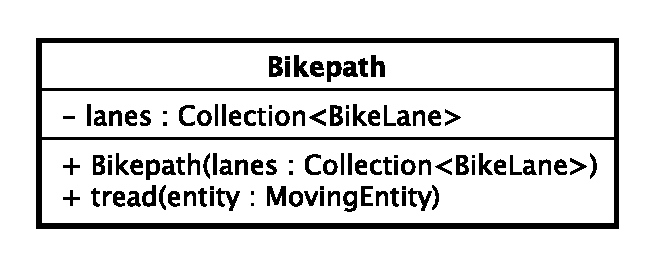
\includegraphics[scale=0.6,keepaspectratio]{images/solution/app/backend/bikepath.eps}
\caption{\pReactiveComponent::components::Bikepath}
\label{fig:sd-app-bikepath}
\end{figure}
\FloatBarrier
\begin{itemize}
  \item \textbf{\descr} \\
    It represents a concrete bikepath which is composed of one or more lanes.
  \item \textbf{\attrs}
  \begin{itemize}
    \item \texttt{lanes: Collection<BikeLane>} \\
A bikepath is composed of lanes.
  \end{itemize}
  \item \textbf{\ops}
  \begin{itemize}
  \item[+] \texttt{Bikepath(lanes : Collection<BikeLane>)} \\
    Creates a path for bikess.
    \item[+] \texttt{tread(traveller: Traveller)} \\
Moves the traveller on the correct lane based on the current traveller route. 
  \end{itemize}
\end{itemize}
